\section{Engine\-Base Class Reference}
\label{classEngineBase}\index{EngineBase@{EngineBase}}
{\tt \#include $<$enginebase.h$>$}

Inheritance diagram for Engine\-Base:\begin{figure}[H]
\begin{center}
\leavevmode
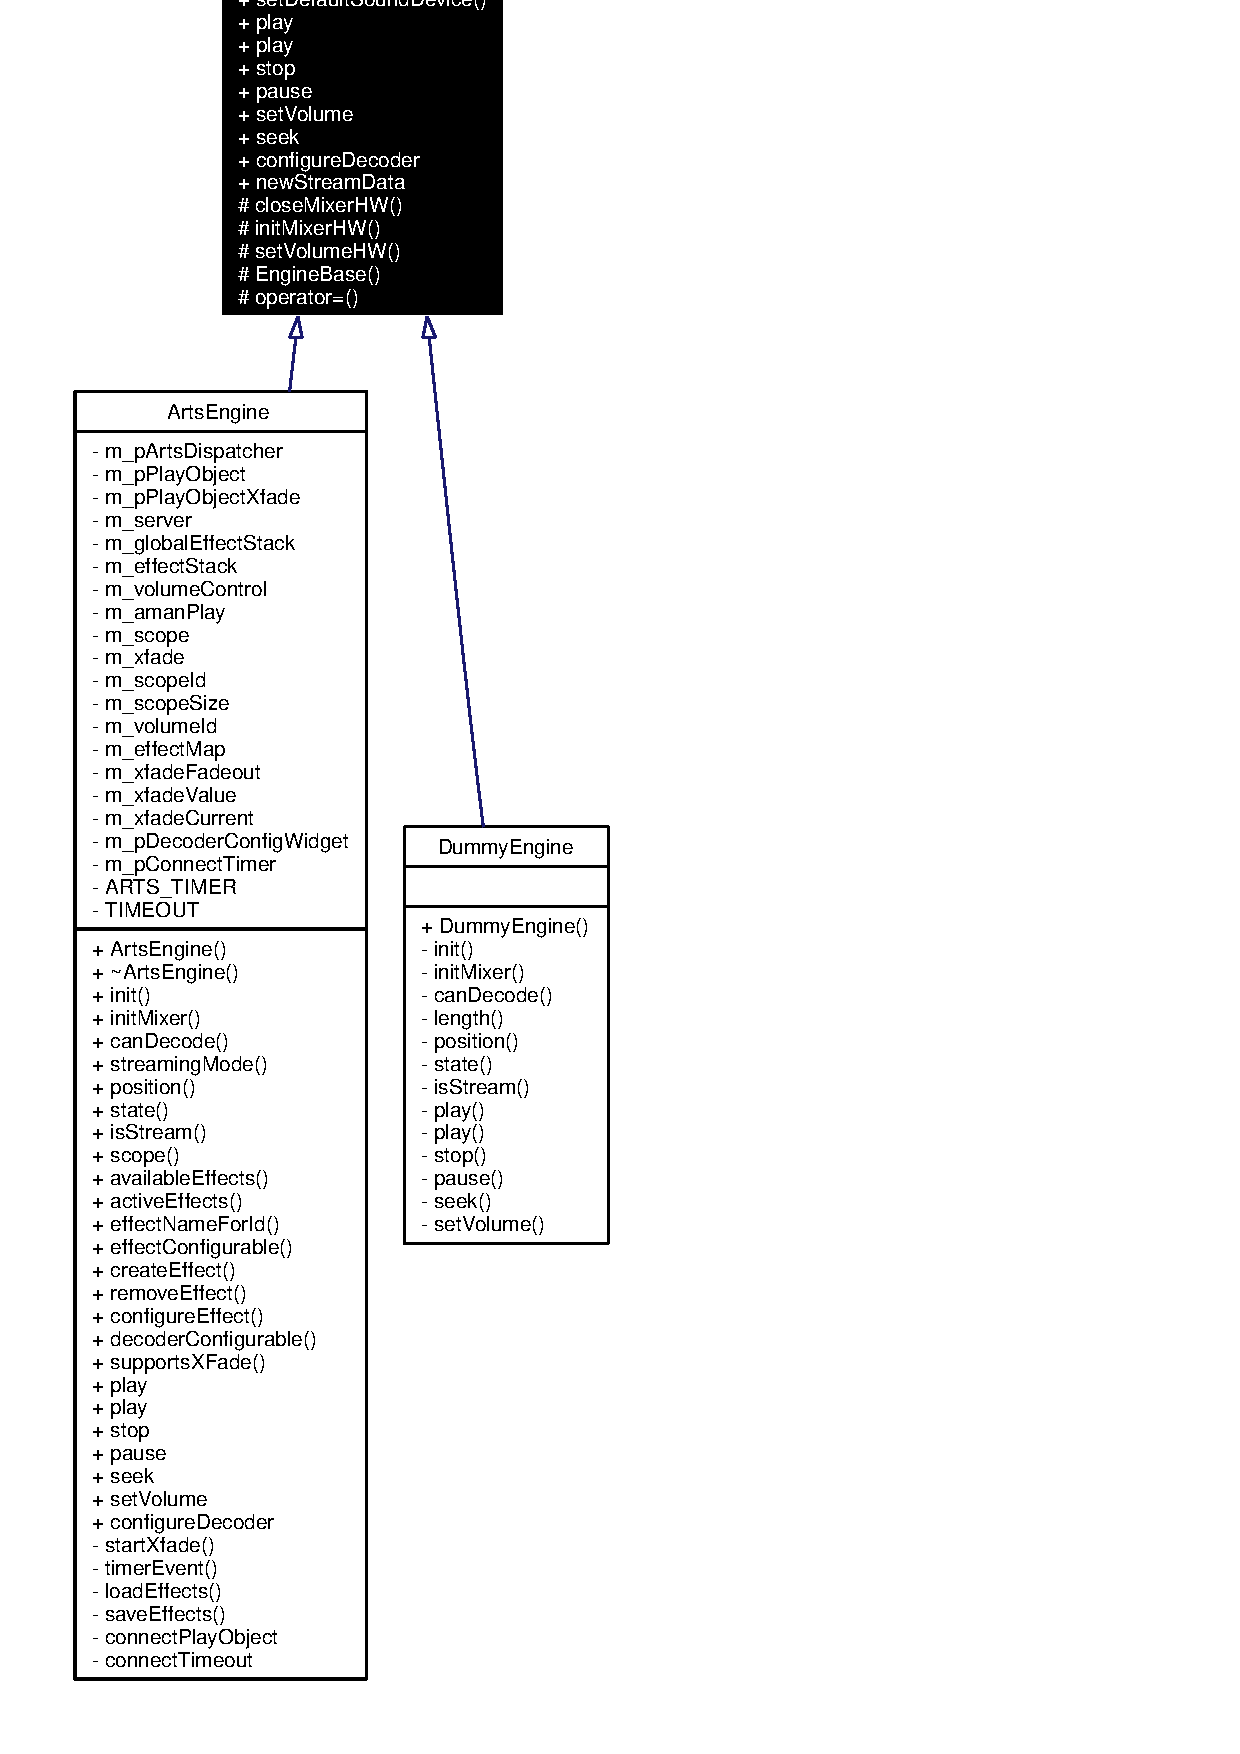
\includegraphics[width=146pt]{classEngineBase__inherit__graph}
\end{center}
\end{figure}
\subsection*{Public Types}
\begin{CompactItemize}
\item 
enum {\bf Engine\-State} \{ {\bf Empty}, 
{\bf Idle}, 
{\bf Playing}, 
{\bf Paused}
 \}
\item 
enum {\bf Streaming\-Mode} \{ {\bf Socket}, 
{\bf Signal}, 
{\bf No\-Streaming}
 \}
\end{CompactItemize}
\subsection*{Public Slots}
\begin{CompactItemize}
\item 
virtual void {\bf play} (const KURL \&)=0
\item 
virtual void {\bf play} ()=0
\item 
virtual void {\bf stop} ()=0
\item 
virtual void {\bf pause} ()=0
\item 
virtual void {\bf set\-Volume} (int percent)=0
\item 
virtual void {\bf seek} (long ms)=0
\item 
virtual void {\bf configure\-Decoder} ()
\item 
virtual void {\bf new\-Stream\-Data} (char $\ast$, int)
\end{CompactItemize}
\subsection*{Signals}
\begin{CompactItemize}
\item 
void {\bf end\-Of\-Track} ()
\item 
void {\bf stopped} ()
\end{CompactItemize}
\subsection*{Public Member Functions}
\begin{CompactItemize}
\item 
{\bf Engine\-Base} ()
\item 
virtual {\bf $\sim$Engine\-Base} ()
\item 
virtual void {\bf init} (bool \&restart, int scope\-Size, bool restore\-Effects)=0
\item 
virtual bool {\bf init\-Mixer} (bool hardware)=0
\item 
virtual bool {\bf can\-Decode} (const KURL \&url, mode\_\-t mode, mode\_\-t permissions)=0
\item 
virtual {\bf Streaming\-Mode} {\bf streaming\-Mode} ()
\item 
virtual QString\-List {\bf get\-Outputs\-List} ()
\item 
virtual long {\bf position} () const=0
\item 
virtual {\bf Engine\-State} {\bf state} () const=0
\item 
bool {\bf loaded} ()
\item 
int {\bf volume} () const 
\item 
bool {\bf is\-Mixer\-Hardware} () const 
\item 
virtual bool {\bf is\-Stream} () const=0
\item 
virtual bool {\bf supports\-XFade} () const 
\item 
virtual std::vector$<$ float $>$ $\ast$ {\bf scope} ()
\item 
void {\bf set\-Restore\-Effects} (bool yes)
\item 
virtual QString\-List {\bf available\-Effects} () const 
\item 
virtual std::vector$<$ long $>$ {\bf active\-Effects} () const 
\item 
virtual QString {\bf effect\-Name\-For\-Id} (long) const 
\item 
virtual bool {\bf effect\-Configurable} (long) const 
\item 
virtual long {\bf create\-Effect} (const QString \&)
\item 
virtual void {\bf remove\-Effect} (long)
\item 
virtual void {\bf configure\-Effect} (long)
\item 
virtual bool {\bf decoder\-Configurable} () const 
\item 
virtual void {\bf set\-Xfade\-Length} (int ms)
\item 
virtual void {\bf set\-Sound\-Output} (const QString \&output)
\item 
virtual void {\bf set\-Sound\-Device} (const QString \&device)
\item 
virtual void {\bf set\-Default\-Sound\-Device} (bool is\-Default)
\end{CompactItemize}
\subsection*{Protected Member Functions}
\begin{CompactItemize}
\item 
void {\bf close\-Mixer\-HW} ()
\item 
bool {\bf init\-Mixer\-HW} ()
\item 
void {\bf set\-Volume\-HW} (int percent)
\item 
{\bf Engine\-Base} (const {\bf Engine\-Base} \&)
\item 
const {\bf Engine\-Base} \& {\bf operator=} (const {\bf Engine\-Base} \&)
\end{CompactItemize}
\subsection*{Protected Attributes}
\begin{CompactItemize}
\item 
int {\bf m\_\-mixer\-HW}
\item 
int {\bf m\_\-volume}
\item 
int {\bf m\_\-xfade\-Length}
\item 
bool {\bf m\_\-restore\-Effects}
\item 
QString {\bf m\_\-sound\-Output}
\item 
QString {\bf m\_\-sound\-Device}
\item 
bool {\bf m\_\-default\-Sound\-Device}
\end{CompactItemize}


\subsection{Member Enumeration Documentation}
\index{EngineBase@{Engine\-Base}!EngineState@{EngineState}}
\index{EngineState@{EngineState}!EngineBase@{Engine\-Base}}
\subsubsection{\setlength{\rightskip}{0pt plus 5cm}enum {\bf Engine\-Base::Engine\-State}}\label{classEngineBase_EngineBasew7}


\begin{Desc}
\item[Enumeration values: ]\par
\begin{description}
\index{Empty@{Empty}!EngineBase@{EngineBase}}\index{EngineBase@{EngineBase}!Empty@{Empty}}\item[{\em 
Empty\label{classEngineBase_EngineBasew7EngineBasew0}
}]\index{Idle@{Idle}!EngineBase@{EngineBase}}\index{EngineBase@{EngineBase}!Idle@{Idle}}\item[{\em 
Idle\label{classEngineBase_EngineBasew7EngineBasew1}
}]\index{Playing@{Playing}!EngineBase@{EngineBase}}\index{EngineBase@{EngineBase}!Playing@{Playing}}\item[{\em 
Playing\label{classEngineBase_EngineBasew7EngineBasew2}
}]\index{Paused@{Paused}!EngineBase@{EngineBase}}\index{EngineBase@{EngineBase}!Paused@{Paused}}\item[{\em 
Paused\label{classEngineBase_EngineBasew7EngineBasew3}
}]\end{description}
\end{Desc}



Definition at line 43 of file enginebase.h.



\footnotesize\begin{verbatim}43 { Empty, Idle, Playing, Paused };
\end{verbatim}\normalsize 
\index{EngineBase@{Engine\-Base}!StreamingMode@{StreamingMode}}
\index{StreamingMode@{StreamingMode}!EngineBase@{Engine\-Base}}
\subsubsection{\setlength{\rightskip}{0pt plus 5cm}enum {\bf Engine\-Base::Streaming\-Mode}}\label{classEngineBase_EngineBasew8}


\begin{Desc}
\item[Enumeration values: ]\par
\begin{description}
\index{Socket@{Socket}!EngineBase@{EngineBase}}\index{EngineBase@{EngineBase}!Socket@{Socket}}\item[{\em 
Socket\label{classEngineBase_EngineBasew8EngineBasew4}
}]\index{Signal@{Signal}!EngineBase@{EngineBase}}\index{EngineBase@{EngineBase}!Signal@{Signal}}\item[{\em 
Signal\label{classEngineBase_EngineBasew8EngineBasew5}
}]\index{NoStreaming@{NoStreaming}!EngineBase@{EngineBase}}\index{EngineBase@{EngineBase}!NoStreaming@{NoStreaming}}\item[{\em 
No\-Streaming\label{classEngineBase_EngineBasew8EngineBasew6}
}]\end{description}
\end{Desc}



Definition at line 44 of file enginebase.h.

Referenced by streaming\-Mode().



\footnotesize\begin{verbatim}44 { Socket, Signal, NoStreaming };
\end{verbatim}\normalsize 


\subsection{Constructor \& Destructor Documentation}
\index{EngineBase@{Engine\-Base}!EngineBase@{EngineBase}}
\index{EngineBase@{EngineBase}!EngineBase@{Engine\-Base}}
\subsubsection{\setlength{\rightskip}{0pt plus 5cm}Engine\-Base::Engine\-Base ()}\label{classEngineBase_EngineBasea0}




Definition at line 30 of file enginebase.cpp.



\footnotesize\begin{verbatim}31 {}
\end{verbatim}\normalsize 
\index{EngineBase@{Engine\-Base}!~EngineBase@{$\sim$EngineBase}}
\index{~EngineBase@{$\sim$EngineBase}!EngineBase@{Engine\-Base}}
\subsubsection{\setlength{\rightskip}{0pt plus 5cm}Engine\-Base::$\sim${\bf Engine\-Base} ()\hspace{0.3cm}{\tt  [virtual]}}\label{classEngineBase_EngineBasea1}




Definition at line 34 of file enginebase.cpp.

References close\-Mixer\-HW().



\footnotesize\begin{verbatim}35 {
36     kdDebug() << k_funcinfo << endl;
37 
38     closeMixerHW();
39 }
\end{verbatim}\normalsize 


Here is the call graph for this function:\begin{figure}[H]
\begin{center}
\leavevmode
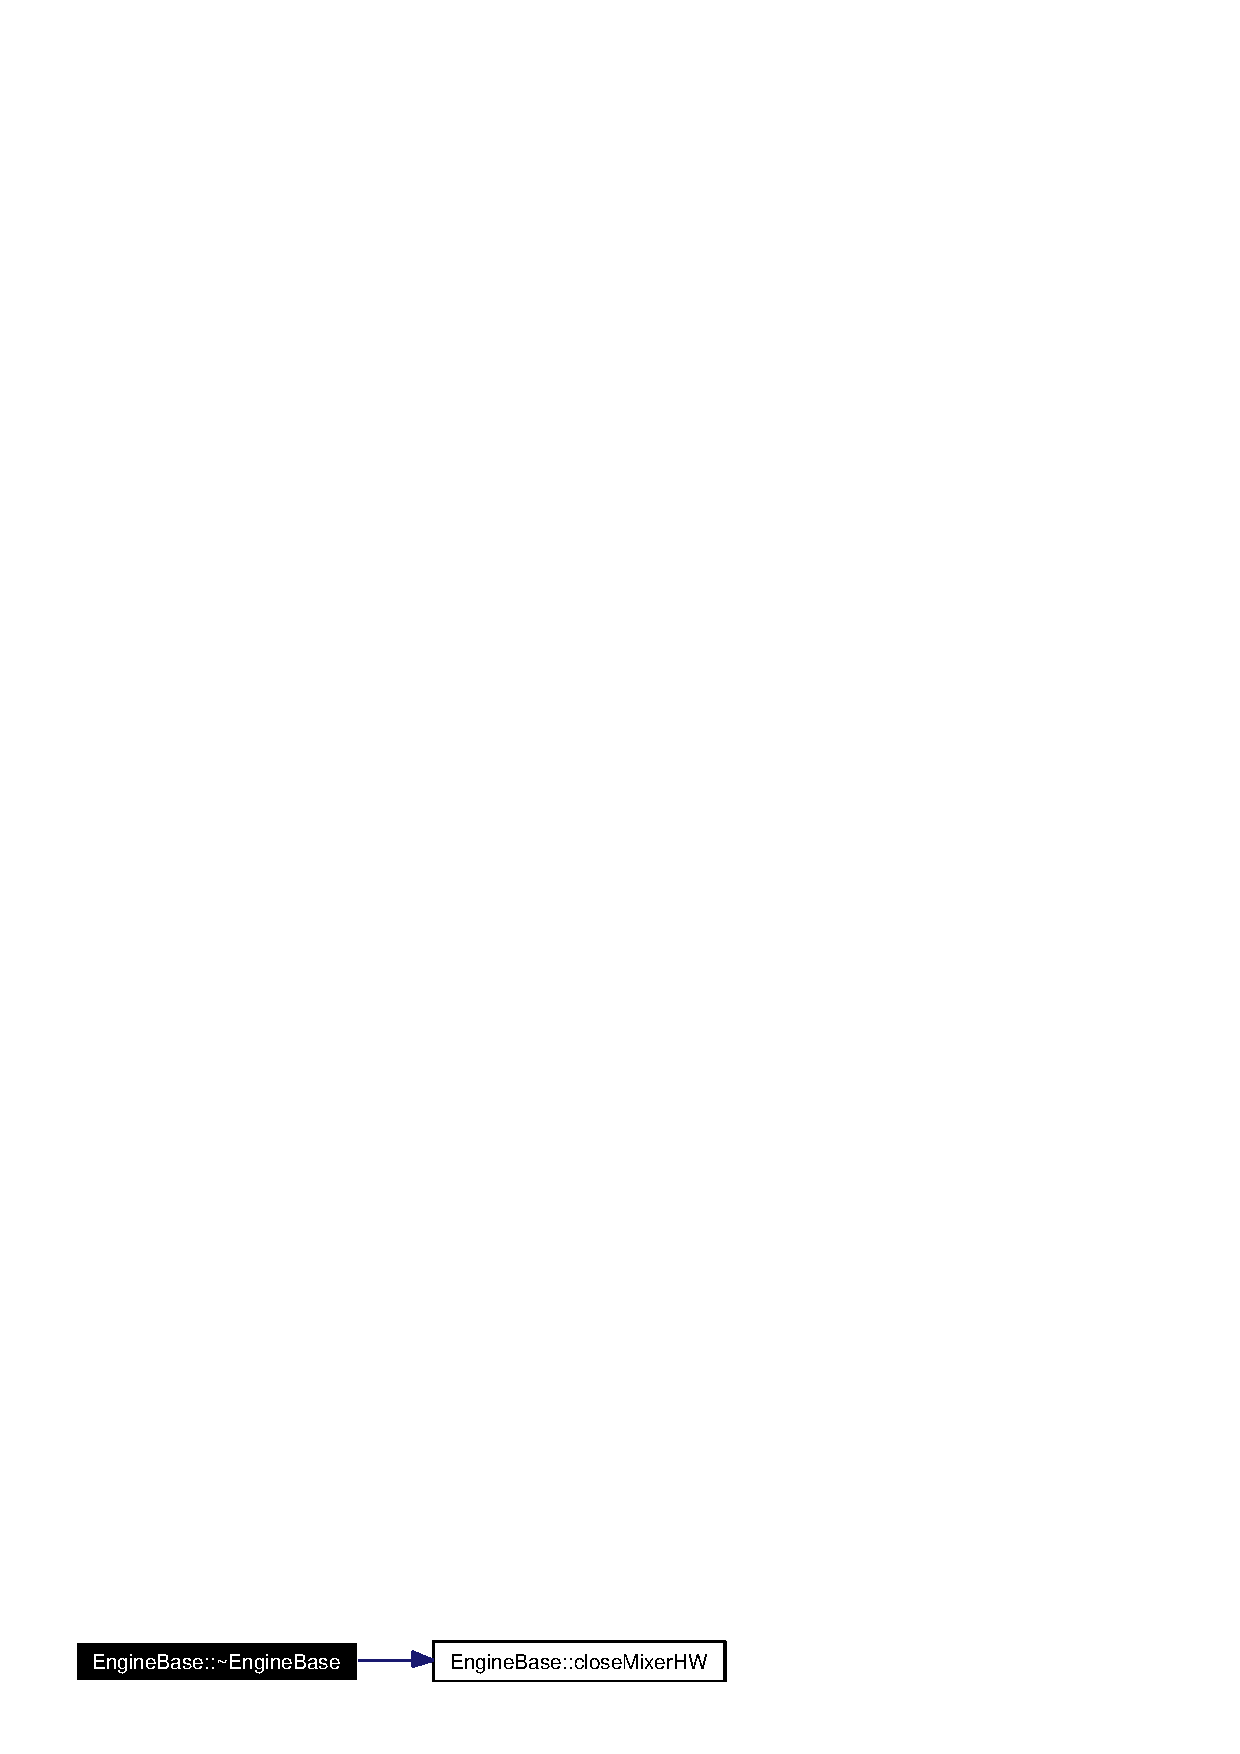
\includegraphics[width=174pt]{classEngineBase_EngineBasea1_cgraph}
\end{center}
\end{figure}
\index{EngineBase@{Engine\-Base}!EngineBase@{EngineBase}}
\index{EngineBase@{EngineBase}!EngineBase@{Engine\-Base}}
\subsubsection{\setlength{\rightskip}{0pt plus 5cm}Engine\-Base::Engine\-Base (const {\bf Engine\-Base} \&)\hspace{0.3cm}{\tt  [protected]}}\label{classEngineBase_EngineBaseb3}




\subsection{Member Function Documentation}
\index{EngineBase@{Engine\-Base}!activeEffects@{activeEffects}}
\index{activeEffects@{activeEffects}!EngineBase@{Engine\-Base}}
\subsubsection{\setlength{\rightskip}{0pt plus 5cm}virtual std::vector$<$long$>$ Engine\-Base::active\-Effects () const\hspace{0.3cm}{\tt  [inline, virtual]}}\label{classEngineBase_EngineBasea17}




Reimplemented in {\bf Arts\-Engine} {\rm (p.\,\pageref{classArtsEngine_ArtsEnginea11})}.

Definition at line 103 of file enginebase.h.



\footnotesize\begin{verbatim}103 { return std::vector<long>(); }
\end{verbatim}\normalsize 
\index{EngineBase@{Engine\-Base}!availableEffects@{availableEffects}}
\index{availableEffects@{availableEffects}!EngineBase@{Engine\-Base}}
\subsubsection{\setlength{\rightskip}{0pt plus 5cm}virtual QString\-List Engine\-Base::available\-Effects () const\hspace{0.3cm}{\tt  [inline, virtual]}}\label{classEngineBase_EngineBasea16}




Reimplemented in {\bf Arts\-Engine} {\rm (p.\,\pageref{classArtsEngine_ArtsEnginea10})}.

Definition at line 102 of file enginebase.h.



\footnotesize\begin{verbatim}102 { return QStringList(); }
\end{verbatim}\normalsize 
\index{EngineBase@{Engine\-Base}!canDecode@{canDecode}}
\index{canDecode@{canDecode}!EngineBase@{Engine\-Base}}
\subsubsection{\setlength{\rightskip}{0pt plus 5cm}virtual bool Engine\-Base::can\-Decode (const KURL \& {\em url}, mode\_\-t {\em mode}, mode\_\-t {\em permissions})\hspace{0.3cm}{\tt  [pure virtual]}}\label{classEngineBase_EngineBasea4}




Implemented in {\bf Arts\-Engine} {\rm (p.\,\pageref{classArtsEngine_ArtsEnginea4})}, and {\bf Dummy\-Engine} {\rm (p.\,\pageref{classDummyEngine_DummyEngined2})}.\index{EngineBase@{Engine\-Base}!closeMixerHW@{closeMixerHW}}
\index{closeMixerHW@{closeMixerHW}!EngineBase@{Engine\-Base}}
\subsubsection{\setlength{\rightskip}{0pt plus 5cm}void Engine\-Base::close\-Mixer\-HW ()\hspace{0.3cm}{\tt  [protected]}}\label{classEngineBase_EngineBaseb0}




Definition at line 61 of file enginebase.cpp.

References m\_\-mixer\-HW.

Referenced by Arts\-Engine::init\-Mixer(), and $\sim$Engine\-Base().



\footnotesize\begin{verbatim}62 {
63     if ( m_mixerHW != -1 )
64     {
65         ::close( m_mixerHW );   //close /dev/mixer device
66         m_mixerHW = -1;
67     }
68 }
\end{verbatim}\normalsize 
\index{EngineBase@{Engine\-Base}!configureDecoder@{configureDecoder}}
\index{configureDecoder@{configureDecoder}!EngineBase@{Engine\-Base}}
\subsubsection{\setlength{\rightskip}{0pt plus 5cm}virtual void Engine\-Base::configure\-Decoder ()\hspace{0.3cm}{\tt  [inline, virtual, slot]}}\label{classEngineBase_EngineBasei6}




Reimplemented in {\bf Arts\-Engine} {\rm (p.\,\pageref{classArtsEngine_ArtsEnginei6})}.

Definition at line 129 of file enginebase.h.



\footnotesize\begin{verbatim}129 {}
\end{verbatim}\normalsize 
\index{EngineBase@{Engine\-Base}!configureEffect@{configureEffect}}
\index{configureEffect@{configureEffect}!EngineBase@{Engine\-Base}}
\subsubsection{\setlength{\rightskip}{0pt plus 5cm}virtual void Engine\-Base::configure\-Effect (long)\hspace{0.3cm}{\tt  [inline, virtual]}}\label{classEngineBase_EngineBasea22}




Reimplemented in {\bf Arts\-Engine} {\rm (p.\,\pageref{classArtsEngine_ArtsEnginea16})}.

Definition at line 108 of file enginebase.h.



\footnotesize\begin{verbatim}108 { }
\end{verbatim}\normalsize 
\index{EngineBase@{Engine\-Base}!createEffect@{createEffect}}
\index{createEffect@{createEffect}!EngineBase@{Engine\-Base}}
\subsubsection{\setlength{\rightskip}{0pt plus 5cm}virtual long Engine\-Base::create\-Effect (const QString \&)\hspace{0.3cm}{\tt  [inline, virtual]}}\label{classEngineBase_EngineBasea20}




Reimplemented in {\bf Arts\-Engine} {\rm (p.\,\pageref{classArtsEngine_ArtsEnginea14})}.

Definition at line 106 of file enginebase.h.



\footnotesize\begin{verbatim}106 { return -1; }
\end{verbatim}\normalsize 
\index{EngineBase@{Engine\-Base}!decoderConfigurable@{decoderConfigurable}}
\index{decoderConfigurable@{decoderConfigurable}!EngineBase@{Engine\-Base}}
\subsubsection{\setlength{\rightskip}{0pt plus 5cm}virtual bool Engine\-Base::decoder\-Configurable () const\hspace{0.3cm}{\tt  [inline, virtual]}}\label{classEngineBase_EngineBasea23}




Definition at line 109 of file enginebase.h.



\footnotesize\begin{verbatim}109 { return false; }
\end{verbatim}\normalsize 
\index{EngineBase@{Engine\-Base}!effectConfigurable@{effectConfigurable}}
\index{effectConfigurable@{effectConfigurable}!EngineBase@{Engine\-Base}}
\subsubsection{\setlength{\rightskip}{0pt plus 5cm}virtual bool Engine\-Base::effect\-Configurable (long) const\hspace{0.3cm}{\tt  [inline, virtual]}}\label{classEngineBase_EngineBasea19}




Reimplemented in {\bf Arts\-Engine} {\rm (p.\,\pageref{classArtsEngine_ArtsEnginea13})}.

Definition at line 105 of file enginebase.h.



\footnotesize\begin{verbatim}105 { return false; }
\end{verbatim}\normalsize 
\index{EngineBase@{Engine\-Base}!effectNameForId@{effectNameForId}}
\index{effectNameForId@{effectNameForId}!EngineBase@{Engine\-Base}}
\subsubsection{\setlength{\rightskip}{0pt plus 5cm}virtual QString Engine\-Base::effect\-Name\-For\-Id (long) const\hspace{0.3cm}{\tt  [inline, virtual]}}\label{classEngineBase_EngineBasea18}




Reimplemented in {\bf Arts\-Engine} {\rm (p.\,\pageref{classArtsEngine_ArtsEnginea12})}.

Definition at line 104 of file enginebase.h.



\footnotesize\begin{verbatim}104 { return QString::null; }
\end{verbatim}\normalsize 
\index{EngineBase@{Engine\-Base}!endOfTrack@{endOfTrack}}
\index{endOfTrack@{endOfTrack}!EngineBase@{Engine\-Base}}
\subsubsection{\setlength{\rightskip}{0pt plus 5cm}void Engine\-Base::end\-Of\-Track ()\hspace{0.3cm}{\tt  [signal]}}\label{classEngineBase_EngineBasel0}




Definition at line 113 of file enginebase.moc.



\footnotesize\begin{verbatim}114 {
115     activate_signal( staticMetaObject()->signalOffset() + 0 );
116 }
\end{verbatim}\normalsize 
\index{EngineBase@{Engine\-Base}!getOutputsList@{getOutputsList}}
\index{getOutputsList@{getOutputsList}!EngineBase@{Engine\-Base}}
\subsubsection{\setlength{\rightskip}{0pt plus 5cm}virtual QString\-List Engine\-Base::get\-Outputs\-List ()\hspace{0.3cm}{\tt  [inline, virtual]}}\label{classEngineBase_EngineBasea6}


Get list of available output plugins 

Definition at line 61 of file enginebase.h.



\footnotesize\begin{verbatim}61 { return QStringList(); }
\end{verbatim}\normalsize 
\index{EngineBase@{Engine\-Base}!init@{init}}
\index{init@{init}!EngineBase@{Engine\-Base}}
\subsubsection{\setlength{\rightskip}{0pt plus 5cm}virtual void Engine\-Base::init (bool \& {\em restart}, int {\em scope\-Size}, bool {\em restore\-Effects})\hspace{0.3cm}{\tt  [pure virtual]}}\label{classEngineBase_EngineBasea2}




Implemented in {\bf Arts\-Engine} {\rm (p.\,\pageref{classArtsEngine_ArtsEnginea2})}, and {\bf Dummy\-Engine} {\rm (p.\,\pageref{classDummyEngine_DummyEngined0})}.

Referenced by Myplayer::Myplayer().\index{EngineBase@{Engine\-Base}!initMixer@{initMixer}}
\index{initMixer@{initMixer}!EngineBase@{Engine\-Base}}
\subsubsection{\setlength{\rightskip}{0pt plus 5cm}virtual bool Engine\-Base::init\-Mixer (bool {\em hardware})\hspace{0.3cm}{\tt  [pure virtual]}}\label{classEngineBase_EngineBasea3}


Initialize mixer. \begin{Desc}
\item[Parameters:]
\begin{description}
\item[{\em hardware}]True for soundcard hardware mixing \end{description}
\end{Desc}
\begin{Desc}
\item[Returns:]True if using hardware mixing \end{Desc}


Implemented in {\bf Arts\-Engine} {\rm (p.\,\pageref{classArtsEngine_ArtsEnginea3})}, and {\bf Dummy\-Engine} {\rm (p.\,\pageref{classDummyEngine_DummyEngined1})}.

Referenced by Myplayer::Myplayer().\index{EngineBase@{Engine\-Base}!initMixerHW@{initMixerHW}}
\index{initMixerHW@{initMixerHW}!EngineBase@{Engine\-Base}}
\subsubsection{\setlength{\rightskip}{0pt plus 5cm}bool Engine\-Base::init\-Mixer\-HW ()\hspace{0.3cm}{\tt  [protected]}}\label{classEngineBase_EngineBaseb1}




Definition at line 43 of file enginebase.cpp.

References m\_\-mixer\-HW.

Referenced by Arts\-Engine::init\-Mixer().



\footnotesize\begin{verbatim}44 {
45     if ( ( m_mixerHW = ::open( "/dev/mixer", O_RDWR ) ) < 0 )
46         return false;  //failed
47     else
48     {
49         int devmask, recmask, i_recsrc, stereodevs;
50         if ( ioctl( m_mixerHW, SOUND_MIXER_READ_DEVMASK, &devmask )       == -1 ) return false;
51         if ( ioctl( m_mixerHW, SOUND_MIXER_READ_RECMASK, &recmask )       == -1 ) return false;
52         if ( ioctl( m_mixerHW, SOUND_MIXER_READ_RECSRC, &i_recsrc )       == -1 ) return false;
53         if ( ioctl( m_mixerHW, SOUND_MIXER_READ_STEREODEVS, &stereodevs ) == -1 ) return false;
54         if ( !devmask )                                                           return false;
55     }
56 
57     return true;
58 }
\end{verbatim}\normalsize 
\index{EngineBase@{Engine\-Base}!isMixerHardware@{isMixerHardware}}
\index{isMixerHardware@{isMixerHardware}!EngineBase@{Engine\-Base}}
\subsubsection{\setlength{\rightskip}{0pt plus 5cm}bool Engine\-Base::is\-Mixer\-Hardware () const\hspace{0.3cm}{\tt  [inline]}}\label{classEngineBase_EngineBasea11}


Sets the master volume. \begin{Desc}
\item[Returns:]True if using hardware mixer. \end{Desc}


Definition at line 85 of file enginebase.h.

References m\_\-mixer\-HW.



\footnotesize\begin{verbatim}85 { return m_mixerHW != -1; }
\end{verbatim}\normalsize 
\index{EngineBase@{Engine\-Base}!isStream@{isStream}}
\index{isStream@{isStream}!EngineBase@{Engine\-Base}}
\subsubsection{\setlength{\rightskip}{0pt plus 5cm}virtual bool Engine\-Base::is\-Stream () const\hspace{0.3cm}{\tt  [pure virtual]}}\label{classEngineBase_EngineBasea12}




Implemented in {\bf Arts\-Engine} {\rm (p.\,\pageref{classArtsEngine_ArtsEnginea8})}, and {\bf Dummy\-Engine} {\rm (p.\,\pageref{classDummyEngine_DummyEngined6})}.

Referenced by Engine\-Controller::slot\-Main\-Timer().\index{EngineBase@{Engine\-Base}!loaded@{loaded}}
\index{loaded@{loaded}!EngineBase@{Engine\-Base}}
\subsubsection{\setlength{\rightskip}{0pt plus 5cm}bool Engine\-Base::loaded ()\hspace{0.3cm}{\tt  [inline]}}\label{classEngineBase_EngineBasea9}


\begin{Desc}
\item[Returns:]True if media is loaded, system is ready to play. \end{Desc}


Definition at line 73 of file enginebase.h.

References Empty, and state().

Referenced by Engine\-Controller::pause().



\footnotesize\begin{verbatim}73 { return state() != Empty; }
\end{verbatim}\normalsize 


Here is the call graph for this function:\begin{figure}[H]
\begin{center}
\leavevmode
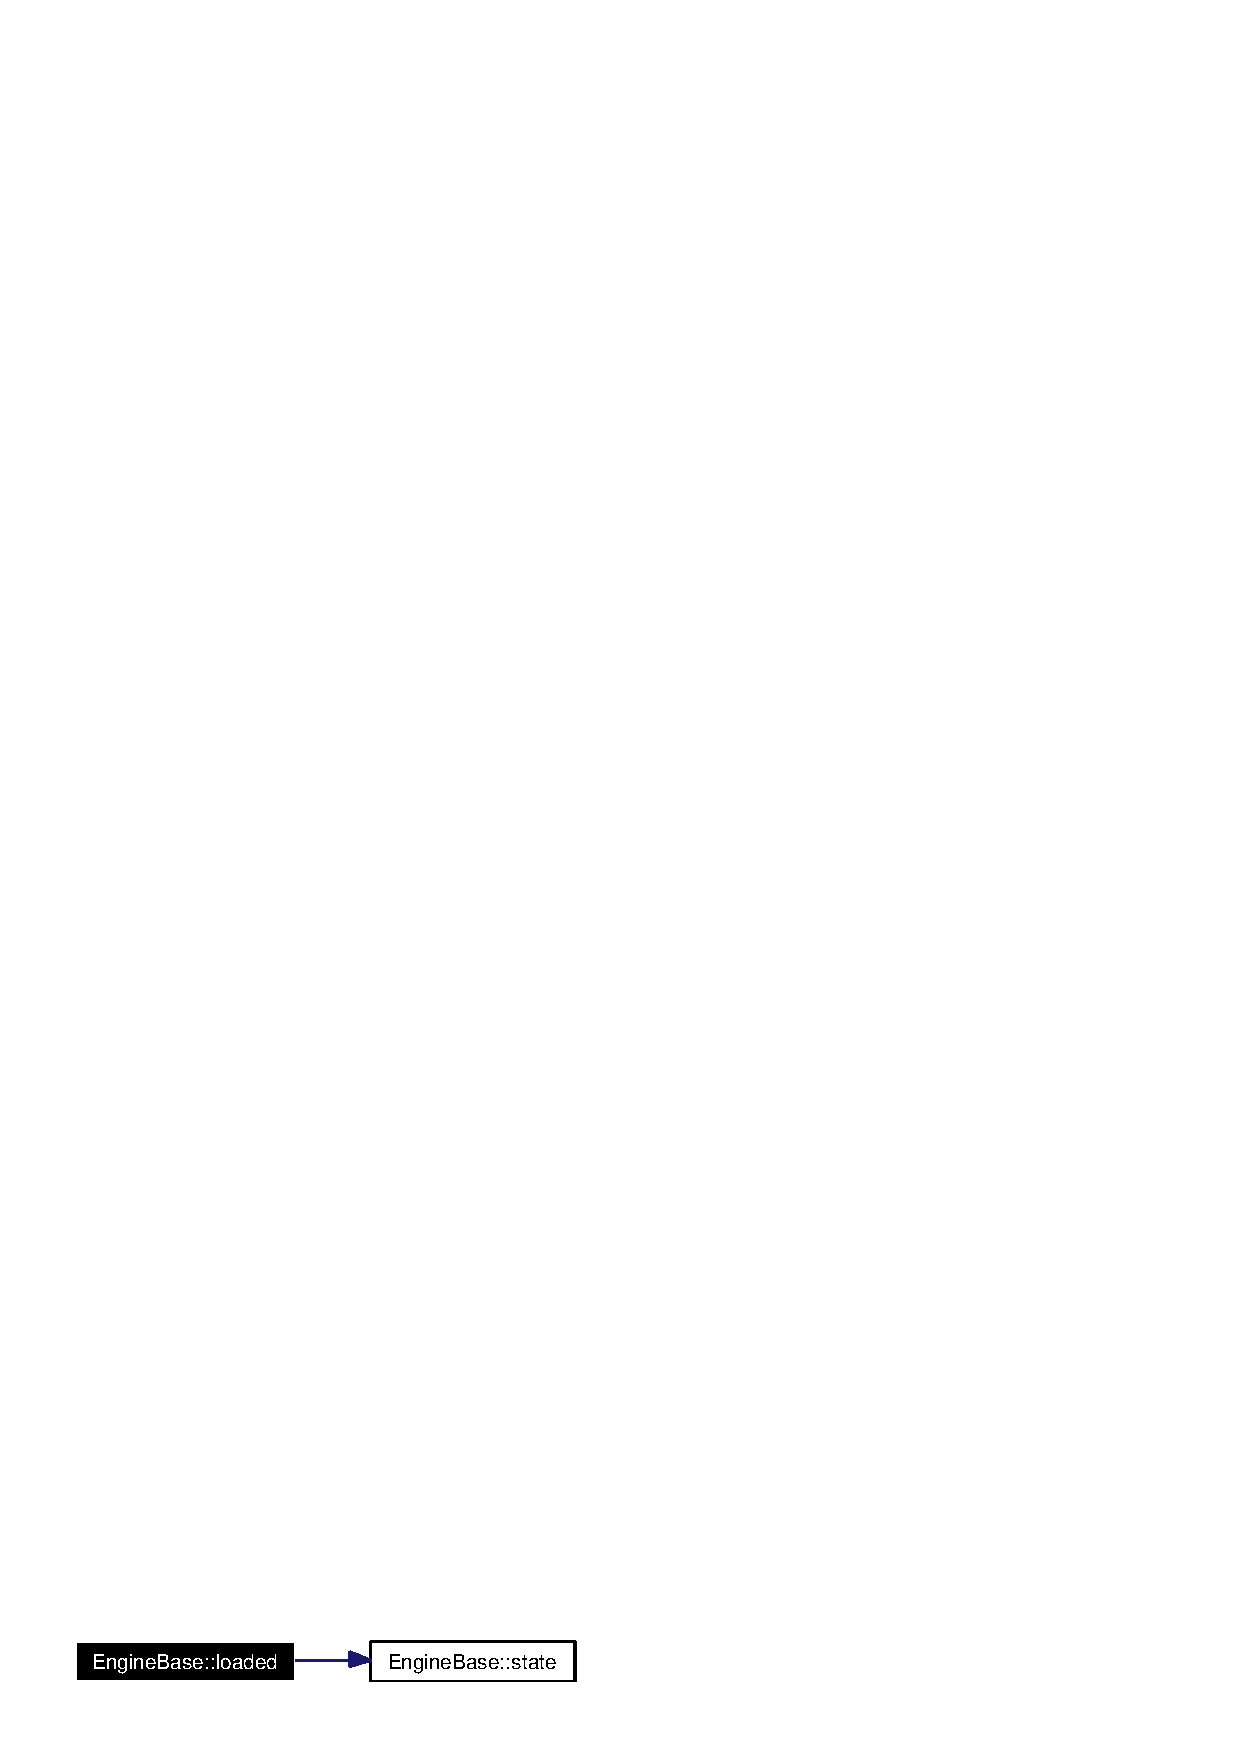
\includegraphics[width=138pt]{classEngineBase_EngineBasea9_cgraph}
\end{center}
\end{figure}
\index{EngineBase@{Engine\-Base}!newStreamData@{newStreamData}}
\index{newStreamData@{newStreamData}!EngineBase@{Engine\-Base}}
\subsubsection{\setlength{\rightskip}{0pt plus 5cm}virtual void Engine\-Base::new\-Stream\-Data (char $\ast$, int)\hspace{0.3cm}{\tt  [inline, virtual, slot]}}\label{classEngineBase_EngineBasei7}




Definition at line 130 of file enginebase.h.



\footnotesize\begin{verbatim}130 {};
\end{verbatim}\normalsize 
\index{EngineBase@{Engine\-Base}!operator=@{operator=}}
\index{operator=@{operator=}!EngineBase@{Engine\-Base}}
\subsubsection{\setlength{\rightskip}{0pt plus 5cm}const {\bf Engine\-Base}\& Engine\-Base::operator= (const {\bf Engine\-Base} \&)\hspace{0.3cm}{\tt  [protected]}}\label{classEngineBase_EngineBaseb4}


\index{EngineBase@{Engine\-Base}!pause@{pause}}
\index{pause@{pause}!EngineBase@{Engine\-Base}}
\subsubsection{\setlength{\rightskip}{0pt plus 5cm}virtual void Engine\-Base::pause ()\hspace{0.3cm}{\tt  [pure virtual, slot]}}\label{classEngineBase_EngineBasei3}




Implemented in {\bf Arts\-Engine} {\rm (p.\,\pageref{classArtsEngine_ArtsEnginei3})}, and {\bf Dummy\-Engine} {\rm (p.\,\pageref{classDummyEngine_DummyEngined10})}.

Referenced by Engine\-Controller::pause().\index{EngineBase@{Engine\-Base}!play@{play}}
\index{play@{play}!EngineBase@{Engine\-Base}}
\subsubsection{\setlength{\rightskip}{0pt plus 5cm}virtual void Engine\-Base::play ()\hspace{0.3cm}{\tt  [pure virtual, slot]}}\label{classEngineBase_EngineBasei1}




Implemented in {\bf Arts\-Engine} {\rm (p.\,\pageref{classArtsEngine_ArtsEnginei1})}, and {\bf Dummy\-Engine} {\rm (p.\,\pageref{classDummyEngine_DummyEngined8})}.\index{EngineBase@{Engine\-Base}!play@{play}}
\index{play@{play}!EngineBase@{Engine\-Base}}
\subsubsection{\setlength{\rightskip}{0pt plus 5cm}virtual void Engine\-Base::play (const KURL \&)\hspace{0.3cm}{\tt  [pure virtual, slot]}}\label{classEngineBase_EngineBasei0}




Implemented in {\bf Arts\-Engine} {\rm (p.\,\pageref{classArtsEngine_ArtsEnginei0})}, and {\bf Dummy\-Engine} {\rm (p.\,\pageref{classDummyEngine_DummyEngined7})}.

Referenced by Engine\-Controller::pause(), and Engine\-Controller::play().\index{EngineBase@{Engine\-Base}!position@{position}}
\index{position@{position}!EngineBase@{Engine\-Base}}
\subsubsection{\setlength{\rightskip}{0pt plus 5cm}virtual long Engine\-Base::position () const\hspace{0.3cm}{\tt  [pure virtual]}}\label{classEngineBase_EngineBasea7}


\begin{Desc}
\item[Returns:]Time position in ms \end{Desc}


Implemented in {\bf Arts\-Engine} {\rm (p.\,\pageref{classArtsEngine_ArtsEnginea6})}, and {\bf Dummy\-Engine} {\rm (p.\,\pageref{classDummyEngine_DummyEngined4})}.

Referenced by Engine\-Controller::slot\-Main\-Timer().\index{EngineBase@{Engine\-Base}!removeEffect@{removeEffect}}
\index{removeEffect@{removeEffect}!EngineBase@{Engine\-Base}}
\subsubsection{\setlength{\rightskip}{0pt plus 5cm}virtual void Engine\-Base::remove\-Effect (long)\hspace{0.3cm}{\tt  [inline, virtual]}}\label{classEngineBase_EngineBasea21}




Reimplemented in {\bf Arts\-Engine} {\rm (p.\,\pageref{classArtsEngine_ArtsEnginea15})}.

Definition at line 107 of file enginebase.h.



\footnotesize\begin{verbatim}107 { }
\end{verbatim}\normalsize 
\index{EngineBase@{Engine\-Base}!scope@{scope}}
\index{scope@{scope}!EngineBase@{Engine\-Base}}
\subsubsection{\setlength{\rightskip}{0pt plus 5cm}virtual std::vector$<$float$>$$\ast$ Engine\-Base::scope ()\hspace{0.3cm}{\tt  [inline, virtual]}}\label{classEngineBase_EngineBasea14}


Fetches the current audio sample buffer. \begin{Desc}
\item[Returns:]Pointer to result of FFT calculation. Must be deleted after use. \end{Desc}


Reimplemented in {\bf Arts\-Engine} {\rm (p.\,\pageref{classArtsEngine_ArtsEnginea9})}.

Definition at line 99 of file enginebase.h.

Referenced by Analyzer::Base$<$ W $>$::draw\-Frame().



\footnotesize\begin{verbatim}99 { return new std::vector<float>(); }
\end{verbatim}\normalsize 
\index{EngineBase@{Engine\-Base}!seek@{seek}}
\index{seek@{seek}!EngineBase@{Engine\-Base}}
\subsubsection{\setlength{\rightskip}{0pt plus 5cm}virtual void Engine\-Base::seek (long {\em ms})\hspace{0.3cm}{\tt  [pure virtual, slot]}}\label{classEngineBase_EngineBasei5}




Implemented in {\bf Arts\-Engine} {\rm (p.\,\pageref{classArtsEngine_ArtsEnginei4})}, and {\bf Dummy\-Engine} {\rm (p.\,\pageref{classDummyEngine_DummyEngined11})}.

Referenced by Myplayer::handle\-Slider().\index{EngineBase@{Engine\-Base}!setDefaultSoundDevice@{setDefaultSoundDevice}}
\index{setDefaultSoundDevice@{setDefaultSoundDevice}!EngineBase@{Engine\-Base}}
\subsubsection{\setlength{\rightskip}{0pt plus 5cm}virtual void Engine\-Base::set\-Default\-Sound\-Device (bool {\em is\-Default})\hspace{0.3cm}{\tt  [inline, virtual]}}\label{classEngineBase_EngineBasea27}




Definition at line 114 of file enginebase.h.

References m\_\-default\-Sound\-Device.

Referenced by Myplayer::Myplayer().



\footnotesize\begin{verbatim}114 { m_defaultSoundDevice = isDefault; }
\end{verbatim}\normalsize 
\index{EngineBase@{Engine\-Base}!setRestoreEffects@{setRestoreEffects}}
\index{setRestoreEffects@{setRestoreEffects}!EngineBase@{Engine\-Base}}
\subsubsection{\setlength{\rightskip}{0pt plus 5cm}void Engine\-Base::set\-Restore\-Effects (bool {\em yes})\hspace{0.3cm}{\tt  [inline]}}\label{classEngineBase_EngineBasea15}




Definition at line 101 of file enginebase.h.

References m\_\-restore\-Effects.

Referenced by Myplayer::Myplayer().



\footnotesize\begin{verbatim}101 { m_restoreEffects = yes; }
\end{verbatim}\normalsize 
\index{EngineBase@{Engine\-Base}!setSoundDevice@{setSoundDevice}}
\index{setSoundDevice@{setSoundDevice}!EngineBase@{Engine\-Base}}
\subsubsection{\setlength{\rightskip}{0pt plus 5cm}virtual void Engine\-Base::set\-Sound\-Device (const QString \& {\em device})\hspace{0.3cm}{\tt  [inline, virtual]}}\label{classEngineBase_EngineBasea26}




Definition at line 113 of file enginebase.h.

References m\_\-sound\-Device.

Referenced by Myplayer::Myplayer().



\footnotesize\begin{verbatim}113 { m_soundDevice = device; }
\end{verbatim}\normalsize 
\index{EngineBase@{Engine\-Base}!setSoundOutput@{setSoundOutput}}
\index{setSoundOutput@{setSoundOutput}!EngineBase@{Engine\-Base}}
\subsubsection{\setlength{\rightskip}{0pt plus 5cm}void Engine\-Base::set\-Sound\-Output (const QString \& {\em output})\hspace{0.3cm}{\tt  [virtual]}}\label{classEngineBase_EngineBasea25}




Definition at line 87 of file enginebase.cpp.

References m\_\-sound\-Output.

Referenced by Myplayer::Myplayer().



\footnotesize\begin{verbatim}88 {
89     kdDebug() << "Setting sound output to: " << output << endl;
90     
91     m_soundOutput = output;
92 }
\end{verbatim}\normalsize 
\index{EngineBase@{Engine\-Base}!setVolume@{setVolume}}
\index{setVolume@{setVolume}!EngineBase@{Engine\-Base}}
\subsubsection{\setlength{\rightskip}{0pt plus 5cm}virtual void Engine\-Base::set\-Volume (int {\em percent})\hspace{0.3cm}{\tt  [pure virtual, slot]}}\label{classEngineBase_EngineBasei4}


\begin{Desc}
\item[Parameters:]
\begin{description}
\item[{\em percent}]Set volume in range 0 to 100. \end{description}
\end{Desc}


Implemented in {\bf Arts\-Engine} {\rm (p.\,\pageref{classArtsEngine_ArtsEnginei5})}, and {\bf Dummy\-Engine} {\rm (p.\,\pageref{classDummyEngine_DummyEngined12})}.

Referenced by Engine\-Controller::Engine\-Controller(), Myplayer::Myplayer(), and Engine\-Controller::set\-Volume().\index{EngineBase@{Engine\-Base}!setVolumeHW@{setVolumeHW}}
\index{setVolumeHW@{setVolumeHW}!EngineBase@{Engine\-Base}}
\subsubsection{\setlength{\rightskip}{0pt plus 5cm}void Engine\-Base::set\-Volume\-HW (int {\em percent})\hspace{0.3cm}{\tt  [protected]}}\label{classEngineBase_EngineBaseb2}




Definition at line 71 of file enginebase.cpp.

References m\_\-mixer\-HW.

Referenced by Arts\-Engine::set\-Volume().



\footnotesize\begin{verbatim}72 {
73     if ( m_mixerHW != -1 )
74     {
75         percent = percent + ( percent << 8 );
76         ioctl( m_mixerHW, MIXER_WRITE( 4 ), &percent );
77     }
78 }
\end{verbatim}\normalsize 
\index{EngineBase@{Engine\-Base}!setXfadeLength@{setXfadeLength}}
\index{setXfadeLength@{setXfadeLength}!EngineBase@{Engine\-Base}}
\subsubsection{\setlength{\rightskip}{0pt plus 5cm}void Engine\-Base::set\-Xfade\-Length (int {\em ms})\hspace{0.3cm}{\tt  [virtual]}}\label{classEngineBase_EngineBasea24}




Definition at line 81 of file enginebase.cpp.

References m\_\-xfade\-Length.

Referenced by Myplayer::Myplayer().



\footnotesize\begin{verbatim}82 {
83     m_xfadeLength = ms;
84 }
\end{verbatim}\normalsize 
\index{EngineBase@{Engine\-Base}!state@{state}}
\index{state@{state}!EngineBase@{Engine\-Base}}
\subsubsection{\setlength{\rightskip}{0pt plus 5cm}virtual {\bf Engine\-State} Engine\-Base::state () const\hspace{0.3cm}{\tt  [pure virtual]}}\label{classEngineBase_EngineBasea8}




Implemented in {\bf Arts\-Engine} {\rm (p.\,\pageref{classArtsEngine_ArtsEnginea7})}, and {\bf Dummy\-Engine} {\rm (p.\,\pageref{classDummyEngine_DummyEngined5})}.

Referenced by Analyzer::Base$<$ W $>$::draw\-Frame(), loaded(), Engine\-Controller::pause(), Engine\-Controller::play(), Engine\-Controller::slot\-Main\-Timer(), and Engine\-Controller::stop().\index{EngineBase@{Engine\-Base}!stop@{stop}}
\index{stop@{stop}!EngineBase@{Engine\-Base}}
\subsubsection{\setlength{\rightskip}{0pt plus 5cm}virtual void Engine\-Base::stop ()\hspace{0.3cm}{\tt  [pure virtual, slot]}}\label{classEngineBase_EngineBasei2}




Implemented in {\bf Arts\-Engine} {\rm (p.\,\pageref{classArtsEngine_ArtsEnginei2})}, and {\bf Dummy\-Engine} {\rm (p.\,\pageref{classDummyEngine_DummyEngined9})}.

Referenced by Engine\-Controller::stop().\index{EngineBase@{Engine\-Base}!stopped@{stopped}}
\index{stopped@{stopped}!EngineBase@{Engine\-Base}}
\subsubsection{\setlength{\rightskip}{0pt plus 5cm}void Engine\-Base::stopped ()\hspace{0.3cm}{\tt  [signal]}}\label{classEngineBase_EngineBasel1}




Definition at line 119 of file enginebase.moc.

Referenced by Arts\-Engine::play().



\footnotesize\begin{verbatim}120 {
121     activate_signal( staticMetaObject()->signalOffset() + 1 );
122 }
\end{verbatim}\normalsize 
\index{EngineBase@{Engine\-Base}!streamingMode@{streamingMode}}
\index{streamingMode@{streamingMode}!EngineBase@{Engine\-Base}}
\subsubsection{\setlength{\rightskip}{0pt plus 5cm}virtual {\bf Streaming\-Mode} Engine\-Base::streaming\-Mode ()\hspace{0.3cm}{\tt  [inline, virtual]}}\label{classEngineBase_EngineBasea5}




Reimplemented in {\bf Arts\-Engine} {\rm (p.\,\pageref{classArtsEngine_ArtsEnginea5})}.

Definition at line 59 of file enginebase.h.

References No\-Streaming, and Streaming\-Mode.



\footnotesize\begin{verbatim}59 { return NoStreaming; }       
\end{verbatim}\normalsize 
\index{EngineBase@{Engine\-Base}!supportsXFade@{supportsXFade}}
\index{supportsXFade@{supportsXFade}!EngineBase@{Engine\-Base}}
\subsubsection{\setlength{\rightskip}{0pt plus 5cm}virtual bool Engine\-Base::supports\-XFade () const\hspace{0.3cm}{\tt  [inline, virtual]}}\label{classEngineBase_EngineBasea13}


Determines whether the engine supports crossfading. \begin{Desc}
\item[Returns:]True if crossfading is supported. \end{Desc}


Reimplemented in {\bf Arts\-Engine} {\rm (p.\,\pageref{classArtsEngine_ArtsEnginea18})}.

Definition at line 93 of file enginebase.h.

Referenced by Engine\-Controller::slot\-Main\-Timer().



\footnotesize\begin{verbatim}93 { return false; }
\end{verbatim}\normalsize 
\index{EngineBase@{Engine\-Base}!volume@{volume}}
\index{volume@{volume}!EngineBase@{Engine\-Base}}
\subsubsection{\setlength{\rightskip}{0pt plus 5cm}int Engine\-Base::volume () const\hspace{0.3cm}{\tt  [inline]}}\label{classEngineBase_EngineBasea10}


Sets the master volume. \begin{Desc}
\item[Returns:]Volume in range 0 to 100. \end{Desc}


Definition at line 79 of file enginebase.h.

References m\_\-volume.

Referenced by Engine\-Controller::decrease\-Volume(), Engine\-Controller::increase\-Volume(), and Engine\-Controller::set\-Volume().



\footnotesize\begin{verbatim}79 { return m_volume; }
\end{verbatim}\normalsize 


\subsection{Member Data Documentation}
\index{EngineBase@{Engine\-Base}!m_defaultSoundDevice@{m\_\-defaultSoundDevice}}
\index{m_defaultSoundDevice@{m\_\-defaultSoundDevice}!EngineBase@{Engine\-Base}}
\subsubsection{\setlength{\rightskip}{0pt plus 5cm}bool {\bf Engine\-Base::m\_\-default\-Sound\-Device}\hspace{0.3cm}{\tt  [protected]}}\label{classEngineBase_EngineBasep6}




Definition at line 145 of file enginebase.h.

Referenced by set\-Default\-Sound\-Device().\index{EngineBase@{Engine\-Base}!m_mixerHW@{m\_\-mixerHW}}
\index{m_mixerHW@{m\_\-mixerHW}!EngineBase@{Engine\-Base}}
\subsubsection{\setlength{\rightskip}{0pt plus 5cm}int {\bf Engine\-Base::m\_\-mixer\-HW}\hspace{0.3cm}{\tt  [protected]}}\label{classEngineBase_EngineBasep0}




Definition at line 139 of file enginebase.h.

Referenced by close\-Mixer\-HW(), init\-Mixer\-HW(), is\-Mixer\-Hardware(), and set\-Volume\-HW().\index{EngineBase@{Engine\-Base}!m_restoreEffects@{m\_\-restoreEffects}}
\index{m_restoreEffects@{m\_\-restoreEffects}!EngineBase@{Engine\-Base}}
\subsubsection{\setlength{\rightskip}{0pt plus 5cm}bool {\bf Engine\-Base::m\_\-restore\-Effects}\hspace{0.3cm}{\tt  [protected]}}\label{classEngineBase_EngineBasep3}




Definition at line 142 of file enginebase.h.

Referenced by set\-Restore\-Effects().\index{EngineBase@{Engine\-Base}!m_soundDevice@{m\_\-soundDevice}}
\index{m_soundDevice@{m\_\-soundDevice}!EngineBase@{Engine\-Base}}
\subsubsection{\setlength{\rightskip}{0pt plus 5cm}QString {\bf Engine\-Base::m\_\-sound\-Device}\hspace{0.3cm}{\tt  [protected]}}\label{classEngineBase_EngineBasep5}




Definition at line 144 of file enginebase.h.

Referenced by set\-Sound\-Device().\index{EngineBase@{Engine\-Base}!m_soundOutput@{m\_\-soundOutput}}
\index{m_soundOutput@{m\_\-soundOutput}!EngineBase@{Engine\-Base}}
\subsubsection{\setlength{\rightskip}{0pt plus 5cm}QString {\bf Engine\-Base::m\_\-sound\-Output}\hspace{0.3cm}{\tt  [protected]}}\label{classEngineBase_EngineBasep4}




Definition at line 143 of file enginebase.h.

Referenced by set\-Sound\-Output().\index{EngineBase@{Engine\-Base}!m_volume@{m\_\-volume}}
\index{m_volume@{m\_\-volume}!EngineBase@{Engine\-Base}}
\subsubsection{\setlength{\rightskip}{0pt plus 5cm}int {\bf Engine\-Base::m\_\-volume}\hspace{0.3cm}{\tt  [protected]}}\label{classEngineBase_EngineBasep1}




Definition at line 140 of file enginebase.h.

Referenced by volume().\index{EngineBase@{Engine\-Base}!m_xfadeLength@{m\_\-xfadeLength}}
\index{m_xfadeLength@{m\_\-xfadeLength}!EngineBase@{Engine\-Base}}
\subsubsection{\setlength{\rightskip}{0pt plus 5cm}int {\bf Engine\-Base::m\_\-xfade\-Length}\hspace{0.3cm}{\tt  [protected]}}\label{classEngineBase_EngineBasep2}




Definition at line 141 of file enginebase.h.

Referenced by set\-Xfade\-Length().

The documentation for this class was generated from the following files:\begin{CompactItemize}
\item 
{\bf enginebase.h}\item 
{\bf enginebase.moc}\item 
{\bf enginebase.cpp}\end{CompactItemize}
